\chapter{Investigating the Intersection of Policing, Place, and Opioids}
%introduction 
% 1. brief contextualization of the opioid od crisis
% 2. role of place in driving od's
% 3. relationship between place, crime, and police
% 4. this may explain police involvment in ods, compared to other first responders 
% 5. but there is little research examining place based explanations of police involvement in od's

%Lit:
%Describe the role of nhood predictors predicting crime and opioid overdoses
%Described literature on why there may be variation in where PD and other first responders respond quicker too

% methods: figures of ods, property crime, violent crime, TPD/TFMR first administration, choropleth maps, then Andreson's S index, descriptive stats of block groups, ml logit looking at incident and nhood predictors for variation btween tpd and tfmr admins.

\section{\centering Introduction}
As opioid overdoses have increased exponentially over the last two decades, the police have increasingly assumed a more complex role in responding to opioid overdoses and administering naloxone to reduce overdose mortality \parencite{quinn_most_2019, ray_national_2023}. While this is not outside of the police mission, it is a change up from how police have traditionally handled substance use issues through arrests (CITES). The police being increasingly outfitted with naloxone means they can be effective in responding to opioid overdoses and reversing opioid overdoses. Importantly, it is crucial to understand how their involvement in responding to opioid overdoses and administering naloxone is influenced by the communities that they serve.

The police tend to operate in communities marked by higher levels of calls for service, crime rates, and disadvantage (CITES). At the same time, public health issues such as opioid overdoses and opioid overdose mortality are spatially concentrated and overlap with communities marked by higher levels of crime and disadvantage as well (CITES). Additionally, police officers tend to outnumber other first responders (CITES). Because public safety issues, namely criminal activity, is a primary responsibility of the police, and because the police are often proactively patrolling, police response ecology differs from other first responders. Thus, the spatial convergence of public health and public safety issues position the police to respond quickly to opioid overdoses and provide immediate and effective life-saving care.

While the spatial overlap of crime and opioid overdoses is fairly well established (CITES), it is less clear if the police do in fact respond to opioid overdoses quicker in these areas. Because public health issues can also overlap with crime and opioid overdoses, emergency medical services (EMS) or other first responders may be well suited to respond quickly as well. Prior work that has looked at where police are more likely to administer naloxone tend aggregate the total rate or count of naloxone administrations or responses to opioid overdoses for police \textit{and} EMS. This research suggests that, together, police and EMS naloxone administrations do concentrate geographically \parencite{heavey_descriptive_2018}. Other work that has attempted to investigate spatial variation in responsiveness indicates that police may be more likely to be first on scene at an overdose in rural areas \parencite{wood_overdose_2021}. However, there are no studies that investigate the spatial variation between first responders at more granular geographic areas like the block group. 

The present study seeks to address this gap in the literature. Using Tempe Fire and Medical Rescue (TFMR) calls for service data I investigate the spatial variation in police administering naloxone first and TFMR administering naloxone first. I use a spatial point pattern test to first descriptively assess if there is variation in where police and TFMR are administering naloxone first across block groups in Tempe, Arizona. Then, because of the nested structure of the data, I employ mixed-effect regression models to assess the incident- and neighborhood-level predictors of police and TFMR administering naloxone first. The findings have implications for policy that guides police discretion and decision-making in opioid overdoses and for community-level programs to expand harm reduction services to improve accessibility of naloxone for community members.

\section{\centering Literature Review}

\subsection{Place, Crime, and Opioid Overdoses}

Early geographical work of the 1800s inspired the contemporary Chicago school which emerged in the early 20th century. The Chicago school is a sociological perspective that explains how the structure of urban life influences outcomes. In one of the earliest tests of the role of urban structure and crime, \textcite{shaw_juvenile_1942} investigated why delinquency was unevenly distributed throughout the city. They found that areas that were socially disorganized – high levels of poverty, racial heterogeneity, and residential instability – experienced higher delinquency rates. \textcite{shaw_juvenile_1942} finding indicated that delinquency was not solely associated with individual-level characteristics, but that structure played a role as well. These findings led to the development of social disorganization theory which suggests that there are neighborhood-level characteristics that influence juvenile delinquency rates regardless of the individual characteristics of those in the neighborhood. One of the primary mechanisms used to explain this finding is that the formation of social ties is hindered in socially disorganized neighborhoods. The systemic model, proposed by \textcite{kasarda_community_1974}, places an emphasis on the social connections between community members \parencite{bursik_jr_economic_1993, bursik_systemic_2000}. Specifically, neighborhoods with strong ties between community members can convey norms, values, and expectations of conduct for the neighborhood. The transmission of these norms and values produces a greater capacity for informal social control among community members \parencite{kornhauser_social_1978}. However, the presence of disadvantage, residential instability, and ethnic heterogeneity can hinder the development of informal social controls. Because there is an inability to develop strong informal social control mechanisms in neighborhoods marked by disadvantage, deviance and other forms of criminal activity can go unthwarted. In one of the first full tests of social disorganization theory, \textcite{sampson_community_1989} showed that there was an indirect effect of neighborhood-level structural characteristics on crime and that the strength of networks among community members mediated the relationship. Contemporary work has continued to support this finding showing the impact of structural characteristics and the role of community ties play across jurisdictions \parencite{bursik_systemic_2000, levy_triple_2020, sampson_great_2012, sampson_neighborhoods_1997}.

Another ecological theoretical framework for explaining the association between community-level characteristics and crime is the macro-level strain theory proposed by \parencite{agnew_robert_general_1999}. Agnew suggests that the differential distribution of crime across communities is not solely a product of weak informal social controls but is a product of the strain producing characteristics in these communities that either blocks individuals’ goals, produces a feeling of deprivation, introduces negative stimuli, or removes positive stimuli. There is also a network effect wherein individuals interact with other highly strained individuals that can impact one’s stress. Communities with strain producing characteristics select strained individuals, particularly for those who are facing economic hardships. These individuals move into the deprived community and are confined to the community because of their inability to relocate. This then leads to community-level differences in crime rates because of the heightened likelihood of a criminal response to the strain experienced in the given neighborhood.

Yet, tests of \textcite{agnew_robert_general_1999} model are relatively limited, particularly at the neighborhood level. Of the research that has been done at the neighborhood level, findings have highlighted the role of strain and its impact on community crime rates \parencite{antunes_social_2022, warner_strain_2003}. This research indicates that strain does play a role in the production of crime rates at the neighborhood level. \textcite{warner_strain_2003} show that the role of informal social controls become statistically non-significant while community-level strain is significantly associated with violence. \textcite{antunes_social_2022} report similar findings in that community level strain, exposure to violence, and youth violence are associated even when controlling for collective efficacy. 

Importantly, the same macro-level process of social disorganization theory and macro-level strain theory that are associated with crime are also associated with opioid overdoses. Community-level characteristics that been found to be associated with overdoses and overdose mortality include higher levels of poverty, ethnic heterogeneity, lower home ownership rates, and low educational attainment \parencite{chichester_pharmacies_2020, galea_income_2003, hannon_neighborhood_2006, ford_neighborhood_2017}. \textcite{ford_neighborhood_2017} show that social disorganization, a lack of social capital, and low social participation are predictive of adolescent opioid misuse. \textcite{winstanley_association_2008} also find the same relationship between social capital and reported opioid dependence. This could suggest that higher levels of social capital indicate greater levels of connectedness with community, family, and school. These findings indicate that stronger ties and social integration is associated with lower levels of reported opioid use. This connectedness likely improves the ability for community members to enact informal social controls and discourage drug use. \textcite{feldmeyer_community_2022} notes that structural factors, which include higher opioid prescription rates, population decline, poor community health, and the loss of manufacturing jobs are associated with higher levels of overdoses. Further, \textcite{feldmeyer_community_2022}findings are in line with the deaths of despair argument proposed by \textcite{case_rising_2015, case_mortality_2017}. Specifically, that the same ecological characteristics are associated with overdose deaths and suicides. \textcite{feldmeyer_community_2022} extend this to show some overlap with homicides as well. In a more recent article looking at drug overdoses in Passaic County, New Jersey from 2015-2019 at the block-group level, \textcite{piza_drug_2023} finds that one of the strongest predictors of drug overdoses is concentrated disadvantage. 

The empirical work investigating the association between structural variables and opioid overdoses suggest that weakened social controls (i.e., lower home ownership rates, population decline, disadvantage) and strain (e.g., loss of employment) influence opioid overdose rates. As discussed above, the formation of ties is important for informal social control. Disadvantage, population decline, and lower homeownership rates are neighborhood characteristics that hinder the formation of social connections which reduces the capacity to develop informal control mechanisms. When informal social control is present, members of a community may discourage opioid use resulting in either less use or potentially less risky use. Also, unemployment and the loss of manufacturing jobs has been found to be associated with elevated opioid overdose rates. This is particularly true for the Appalachian region of the US where many hard labor jobs have become obsolete \parencite{mclean_theres_2016} This association suggests there is a relationship between strain and opioid overdoses. Particularly for communities facing loss of employment opportunities and economic decline. Individuals may be strained because of their inability to achieve monetary goals and are unable to relocate given a variety of reasons including their economic situation. Communities facing economic hardships produce strain and retain strained individuals, which then leads to various forms of coping which could be opioid usage \parencite{monnat_factors_2018, monnat_contributions_2019} While these findings suggest that policies should be implemented at the macro-level to address disadvantage, economic decline, and job loss to help facilitate the development of informal social control and reduce strain, there is a practical implication of this overlap between macro-level characteristics, crime, and opioid overdoses. Namely, the potential for police to have an important role in reducing harm in the opioid overdose crisis given that they are also unevenly distributed throughout a city in areas of disadvantage, with higher rates of opioids overdoses, and higher rates of crime.

\subsection{Place and Policing}

Police work is often tied to space and time \parencite{fyfe_police_1991}. Police patrol and activity often reflects local crime trends and areas marked by disadvantage. Across cities, crime – particularly violent crime – tends to be concentrated in neighborhoods characterized by socioeconomic disadvantage \parencite{peterson_divergent_2010}. And the distribution of disadvantage and crime in a city is not random \parencite{rothstein_color_2017, weisburd_law_2015} which highlights the spatial concentration of criminal activity. 

Due to disadvantage, calls for service, crime, and public health related issues being spatially concentrated, police are likely to be situated in these areas frequently \parencite{engel_race_2012, mitchell_criminal_2011}. Deploying police resources based on need – defined as volume of calls for service – is the underpinning of the “deployment hypothesis” \parencite{alexander_war_2010, beckett_penal_2010}. Police departments have attempted to maximize the utility of their limited resources by having officers focus on high-crime areas \parencite{skogan_fairness_2004, weisburd_reforming_2003}. Police activity being spatially concentrated suggests they are positioned to respond to overdoses in places and for populations that may differ from other first-responders, given their availability and patrolling patterns. This is an important aspect of police work that is often overlooked when thinking about their role in responding to public health issues such as the opioid overdose crisis. It has been shown that the police are reaching different communities than EMS for calls for service pertaining to violence and drug activity \parencite{hibdon_concentration_2017, hibdon_going_2021}. Likewise, they may be able to reach overdose incidents prior to EMS or the fire department which could be indicative of a quicker response time in these areas \parencite{pourtaher_naloxone_2022, white_leveraging_2022}. Debates about the role of the police responding to opioid overdoses typically embody a philosophical argument or one that focuses on iatrogenic effects of the police involvement \parencite{doe-simkins_whose_2022, michaud_therapeutic_2023, van_der_meulen_thats_2021}. However, this spatial component of police work as it relates to the opioid overdose crisis suggests the police may be able to administer naloxone and act as a conduit to services in areas where other first responders may infrequently respond to or are delayed in responding. 

\subsection{Policing Opioid Overdoses}

Specifically related to opioids, there is some research that suggests the police may be more likely to respond first to an OD in rural areas \parencite{wood_overdose_2021}. \textcite{pourtaher_naloxone_2022} also find that police are frequently first on scene at an OD in the state of New York. In rural areas resources for other first-responders may be insufficient and response times may be delayed which may explain this finding. Moreover, in Tempe, Arizona, when police respond to a suspected opioid overdose, they are frequently first \parencite{white_leveraging_2022}. But at a more granular level (e.g., neighborhoods), is there variation in police responding to opioid overdoses and administering naloxone? And if there is variation, what is predicting this variation?

At the incident-level, the 911 call description may also influence who responds first. For instance, \textcite{atkins_disparities_2024} show that describing an overdose event as a "non-overdose" was more prevalent when the victim was Black or a female. The authors suggest this could be due to a fear of police response and the potential for an arrest. Prior work has highlighted this fear is prevalent in Black communities \parencite{wagner_post-overdose_2019} and that the general fear of arrest can deter calling 911 \parencite{van_der_meulen_thats_2021}. Moreover, in communities where drug use and specifically opioid use is more prevalent, this avoidance of using certain terminology could have an influence in the aggregate as some harm reduction organizations have advocated for using other terminology than "overdose" when calling 911 to avoid a police response \parencite{zagorski_how_2021}.

However, there is essentially no research on the spatial predictors of police involvement in opioid overdoses outside of the urban/rural divide. It has only been discussed from a theoretical perspective. The present study seeks to address this gap in the literature. 

\section{Current Study}

I am interested in examining if there is a) spatial variation in where police administer naloxone first at the scene of an opioid overdose, and b) why this variation exists. To evaluate the spatial determinants of police administering naloxone, I investigate two research questions:

1) Is there spatial variation, at the block group, in where police administer naloxone first at the scene of an opioid overdose? 

\begin{flushleft}
\(H1_a\): Police administering naloxone first at an opioid overdose incident will vary spatially across block groups. 
\end{flushleft}

2) Why is there spatial variation in where police are more likely to administer naloxone across block groups? 

\begin{flushleft}
\(H2_a\): The violent crime rate at the block group will be associated with a higher likelihood of police administering naloxone first at an opioid overdose incident.
\end{flushleft}

To answer these research questions, I use administrative data from Tempe Fire and Medical Rescue (TFMR) that contains calls for service to opioid related incidents. Importantly, there is an indicator of who administered naloxone prior to TFMR response -- see below for a thorough description of the data. To answer the above research questions, I employ a spatial point pattern test to assess spatial variation in where police are administering naloxone. Second, I employ a mixed-effects logistic regression model with month and year fixed effects to control for unobserved time varying confounders (e.g., seasonality, COVID-19, staffing shifts) to assess incident-level and block-group predictors of where police are more likely to administer naloxone first.

\section{Methods}
\subsection{Setting}

Since 2020 the Tempe Police Department (TPD) has been involved in a collaborative effort with a social services organization – La Frontera EMPACT – to reduce opioid overdose fatalities in Tempe, Arizona. This project, called the Tempe First-Responder Opioid Recovery Project, is funded by the Substance Abuse and Mental Health Services Administration (SAMHSA). The project trained and outfitted Tempe officers with naloxone in January of 2020 and created a 24/7 crisis hotline which officers contacted following an overdose incident to get in contact with a peer navigator (e.g., social outreach worker). Within days of the incident the peer navigator meets with the overdose survivor and their family/friends to provide information regarding potentially useful services (e.g., counseling, drug rehabilitation, housing information, transportation, etc.). Tempe officers have responded to more than 300 overdose incidents during the project. They have administered naloxone over 250 times in which it aided in a successful reversal of opioid overdose symptoms, and they have contacted the 24/7 crisis hotline approximately the same number of times. 

\subsection{Data}
The original data set from TFMR contained 3,257 calls for service to an opioid related incident from 2017-2023. Data on TFMR calls for service to opioid related incidents can be pulled from \href{https://data.tempe.gov/datasets/2daeeafd2741494c8294ca415e5a793e_0/explore?location=33.398962%2C-111.931850%2C11.94}{Tempe.gov}.\footnote{Through a contact at TFMR I was able to obtain other variables -- in addition to the public dataset -- such as the dispatched complaint and whether it was a fatal or nonfatal overdose.} I then geocoded this data set in \texttt{R} using the package \texttt{tidygeocoder} where I specified ArcGIS services as the method for geocoding.\footnote{The geocoding process provides a score that captures how closely an observation matches an address. It ranges from 0 to 100. Of the 3,257 opioid overdose calls for service, the lowest score in the dataset was 79.0\% and overall, there was a mean matching score of 98.6\%.} I then spatially clipped the incident data to a Tempe boundary shapefile (n = 3,207). 

Next, I used the \texttt{tidycensus} package in \texttt{R} where I specified the specific block group variables I am interested in. I used the \texttt{getacs} command to obtain 5-year estimates (2018-2022) for block groups in Tempe, Arizona -- the specific variables will be discussed below. Then, I remove observations where the block group total population estimate is 0 (n = 3,143) -- this also drops 2 block groups (n = 115). Lastly, I remove observations prior to 2020 and the observations in November of 2023 (n = 2,000). 

The offense data is pulled from \href{https://data.tempe.gov/datasets/1563be5b343b4f78b1163e97a9a503ad_0/explore?location=32.279019%2C-112.767075%2C7.97}{Tempe.gov}. The original dataset includes 320,991 observations. I began by limiting the dataset to the pertinent time period (Jan 2020 - Oct 2023; n = 102,681). I then specified three particular crime categories: violent crimes, property crimes, and drug offenses -- these specific categories will be described below. Then, I spatially clip the offenses data to the Tempe boundary shapefile (n = 101,534). 

\subsection{Dependent Variable}
There are two primary dependent variables for the present study: First, a dichotomous variable indicating whether law enforcement administered naloxone first at the scene of an opioid overdose. The final sample includes 288 observations (14.40\%) where law enforcement administered naloxone. There are 1,712 observations (85.60\%) where naloxone was either not administered at all, or naloxone was administered by someone other than law enforcement (e.g., layperson, TFMR, Unknown). I then have a dichotomous variable indicating whether TFMR administered naloxone first compared to all other outcomes(e.g., no administration, PD, layperson, etc.\footnote{As a sensitivity check I collapse this outcome variable on law enforcement and TFMR only. This results in 288 law enforcement administrations (30.22\%) and 665 TFMR administrations (69.78\%). This changes the reference category to more specifically assess variation between these two first-responders. The results do not change.}

\subsection{Independent Variable}
The primary independent variable of interest is the violent crime rate per 1000 residents at the block group. This variable is captured by summing incidence of homicide, manslaughter, aggravated assault, robbery, and burglary with force, dividing by the ACS 5-year population estimate and multiplying by 1000.

I control for both incident level and block group level predictors. At the incident-level I control for the initial dispatch complaint. This variable has 31 different entries. I code them into a  categorical variable that has six values. I separate them into \textit{overdose/poisoning}, \textit{health/medical related}, \textit{accidental injury}, \textit{public safety related}, \textit{mental health related} and \textit{other}.\footnote{Other includes vague and unknown descriptions such as: unconscious/fainting, other, unknown, welfare check, and medical alarm.} I also control for the sex of the individual (= 1 for female [male = 0]). At the block group level I control for drug offense rate,\footnote{Comprised of drug paraphernalia, possession/sell/manufacture of narcotics, and possession/manufacture of prescription drugs offenses.} opioid overdose rate logged, and a series of spatial lags calculated using the spatial weight matrix (\textit{W}) to account for nearby block groups violent crime, drug offenses, and opioid overdose incidents. Additionally, I control for the percentage of residents that are unemployed, non-Hispanic Black, non-Hispanic White, and Hispanic. I also control for the percent of land that is residential \footnote{This was calculated by using the \texttt{osmdata} package in \texttt{R} that allows for the pulling of specific land use features (e.g., bus stops, liquor stores, parks, residential land, etc.). Pulling this data provided a calculation for how much residential land was in Tempe, Arizona. Then, I spatially clipped this to the block group, where I then calculated the percent of residential land by dividing the land use that was residential by the total land in the block group, then multiplying by 100.} and the percent of owner occupied units. Lastly, I incorporate month and year fixed effects to account to time-varying confounders such as seasonality, impacts of COVID-19, and broader year-to-year shifts such as changes in employment levels.\footnote{As a sensitive check I also incorporate day of month fixed effects to account for potential variation across days and weeks, the results do not change.}

\subsection{Analytical Sample}
The final sample includes 2,000 calls for service to opioid overdose incidents from January 2020 through October 2023, nested within 115 block groups in Tempe, Arizona.

\subsection{Analytical Plan}
\subsubsection{Spatial Point Pattern Test}

First, to descriptively assess the spatial variation in PD and TFMR naloxone administrations I employ a spatial point pattern test \parencite{andresen_testing_2009}. This approach compares the pattern of two (or more) outcomes across spatial units (e.g., cell grids, blocks, block groups, police precincts, etc.). It has been applied in a variety of contexts such as crime concentration, police foot patrols, and others (CITES). Specifically related to the present study, I am interested in understanding which block groups experience a higher volume of TPD administering naloxone first on scene at an opioid overdose compared to TFMR. Thus, I have two outcomes of interest to compare spatially. 

The spatial point pattern test works by first identifying which outcome is the base data and which is the test data. Here, the TFMR naloxone administrations are the base data and the PD administrations are the test data. Then, 85\% of the test data is randomly sampled (with replacement) and undergoes Monte Carlo simulations (n = 200). Next, the percentages of points identified within in each block group can be ranked which is then used to remove the top 2.5\% and bottom 2.5\%. This allows for the creation of a 95\% confidence interval around the percentage of the points in each block group. The base data is finally compared to the test data. If the base data falls within the confidence interval, then the two spatial point patterns are similar.

The spatial point pattern analysis can be represented as such:

\[
    S = \frac{\sum_{i=1}^n S_i}{n}
\]

\noindent Where \(n\) is the number of block groups and \(S_i\) is equal to one if the point patterns are similar for block group \(i\). This then produces two \(S\) values. A global \(S\) and robust \(S\). The former refers to a similarity index for all block groups even if the test data was not observed in the spatial units. The latter, however, limits the similarity index to block groups with at least one observation from the test data. 

\subsubsection{Mixed-effects Logistic Model}
To examine why there may be spatial variation in where police and TFMR are administering naloxone first, I employ a multilevel logistic models to handle the nested structure of the data. Specifically, opioid overdose incidents nested within block groups. The equation for this model is as follows:

\[
\text{logit}\left(P(Y_{ij} = 1)\right) = \beta_0 + \sum_{k} \beta_k X_{ij} + \delta_m \text{Month}_{ij} + \lambda_y \text{Year}_{ij} + u_j
\]

\noindent Where \(P(Y_{ij} = 1)\) represents the probability that police or TFMR administer naloxone first at incident \(i\) in block group \(j\). Then, \(\text{logit}(P)\) represents the log odds of police or TFMR administering first. \(\beta_0\) is the intercept and \(\sum_{k} \beta_k X_{ij}\) represents the sum of all fixed effects incident and block group predictor variables. \(\delta_m \text{Month}_{ij}\) and \(\lambda_y \text{Year}_{ij}\) represent month and year fixed effects, respectively. Lastly, \(u_j\) represents the random intercept of block group \(j\).

\section{Results}

Figure 1 depicts the results from the spatial point pattern analysis. Visually, it is clear that TFMR administering naloxone first is less concentrated and more prevalent in Southern Tempe (represented by the blue block groups). The standard \textit{S}-index is .378 and the robust \textit{S}-index is .327 (see table 2). To reiterate, an \textit{S}-index of 1 indicates perfect similarity and 0 perfect dissimilarity. Both similarity indices are in the .3 to .4 range which does indicate that there is spatial variation in where police are administering naloxone first compared to TFMR thus the first null hypothesis can be rejected.

Table 2 presents the results from the main mixed-effects logistic regression models. Police were less likely to administer naloxone first in block groups with higher violent crime rates (OR = 0.997 [.996, .998]). Here, I fail to reject the second null hypothesis. Additionally, police were less likely to administer naloxone first when the initial call for service was described as a health/medical issue (OR = .684 [.507,.920]), a mental health issue (OR = .391 [.241, .6320]), and other (OR = .649 [.4685, .898] compared to an "overdose/poisoning" description. Percentage of owner occupied units is negatively associated with police administering naloxone first (OR = .978 [.960, .995]). On the other hand, there were two block group predictors that were associated with higher odds of a police naloxone administration: drug offense rate (OR = 1.007 [1.004, 1.010]) and percent non-Hispanic Black (OR = 1.025 [1.011, 1.039]).

The violent crime rate at the block group was associated with TFMR being more likely to administer naloxone first (OR = 1.001 [1.000, 1.002]) granted both for police and TFMR these are small substantive differences. TFMR was more likely to administer naloxone first when the intial call for service was described as a health/medical issue (OR = 1.326 [1.013, 1.734]), a mental health issue (OR = 1.998 [1.396, 2.858]), and other (OR = 2.948 [ 2.152, 4.038] compared to an "overdose/poisoning" description. Lastly, drug offense rate was associated with a lower likelihood of TFMR administering naloxone first (OR = .994, [.991, .997]). Figure 2 provides a visualization of the statistically significant coefficients. Panel A provides a look at block group predictors and panel B provides a look at dispatch type.

Table 3 provides the results of the mixed-effects logistic regression model focused solely on police administering first compared to TFMR administering first. More specifically, the reference group is now TFMR administering naloxone first. The results do not substantively change from table 2 although the association between percentage owner occupied units is now marginally significant (\textit{p} < .10). See figure 3 for a visualization of the coefficients.

\section{\centering Discussion}
% contextualize
The present study uses spatial point pattern testing and multi-level logistic regression models to investigate spatial variation in where police and TFMR are administering naloxone first at opioid overdose incidents. There is a limited body of research examining spatial variation in police and other first responders involvement in opioid overdoses, particularly for smaller geographical areas. To my knowledge, the present study is the first to do so at a more granular geographical level. 

% interpret
The results from the spatial point pattern analysis suggest that that there is variation in where police officers are administering naloxone first compared to TFMR. Although this test does not tell use why this variation exists, prior research that discusses variation in hot spots of drug activity for PD and EMS data \parencite{hibdon_concentration_2017, hibdon_going_2021} and the deployment of police to areas with higher levels of calls for service and crime \parencite{engel_police_2003} provides a foundation as to why police may be administering in different areas. The \textit{S}-index in the present study is similar to \textcite{hibdon_concentration_2017}'s similarity index where they found that EMS and PD calls for drug activity overlapped between 24\% and 36\% of the time, although, they were looking at street segments. 

Next, the results from the mixed-effects logistic regression models provide some context for when and where police are more likely and less likely to administer naloxone first. 
% how does violent crime assoc make sense?
The association between the violent crime rate and who administered naloxone first is not in the direction I hypothesized. And although the estimates are statistically significant, substantively, they are small coefficients. Specifically, violent crime rate is associated with a 0.3\% decrease in the odds of police administering first. Nonetheless, one potential explanation for this finding is that violent crimes are likely to produce a police and medical response because someone was likely seriously injured. 

Regarding the initial call dispatch, compared to an overdose description, police are less likely to administer naloxone first when it is health or medical related, mental health related, or other. This is not a surprising finding as health related calls are going to be prioritized by TFMR. This finding also provides partial evidence for the position of some harm reduction agencies to avoid terms that may produce a police response \parencite{zagorski_how_2021}. However, because I am looking at \textit{who administered first} police could still have arrived on scene after TFMR administered naloxone. While this was not tested in the present study, if TFMR is delayed in responding or 911 callers do use specific verbiage to avoid a police response that may be quicker, it could deprive the victim of immediate life-saving care which could contribute to brain damage or death \parencite{winstanley_neurocognitive_2021}. This speaks to the need for police to have formal and informal policies that clearly guide police decision-making to treat drug overdoses as a public health issue to prevent callers from fearing a police response.

% drug offense rate
Additionally, the drug offense rate in the block group was associated with an increase in the odds of police administering naloxone first. Police officers may be frequently patrolling or nearby areas marked by drug activity. In this scenario, it makes sense that they are at the scene of an opioid overdose and administer naloxone first given their proximity to the issue. Unfortunately, the present study cannot parse out the relationship between block group drug offense rates and police administering naloxone first, temporally. Future research should more closely examine this issue longitudinally. Namely, researchers should examine how neighborhood characteristics influence police response over time and ideally can link overdose data to arrest data at the incident-level. At the incident-level, the results from \textcite{white_leveraging_2022} suggest that during the same approximate the same time frame, police in Tempe infrequently made arrests at the scene of a suspected opioid overdose.

% perc owner occ units
Also, the percent of owner occupied units in the block group was associated with a decrease in the odds of police administering naloxone first in table 1 but a marginally significant decrease in table 2. This indicates that police are more likely to administer naloxone first in areas with higher-levels of renter-occupied units or vacant units. Together, renter-occupied and vacant units indicate lower levels of informal social control and more opportunity for criminal activity and drug use. Prior research has highlighted how renter-occupied units indicate a level of instability and lack of informal social control (CITES) which hinders community members willingness to intervene in devious acts (CITES). Further, because of the relationship between a lack of informal control and crime, police officers tend to act as a formal mechanism for control in these areas (CITES). Thus, they may be positioned to respond and administer naloxone first at opioid overdose incidents in these areas.

% black
Lastly, the percent of non-Hispanic Black residents in the block group was associated with an increase in the odds of police administering naloxone first. Given the empirical literature on policing, race, and place, it is not surprising that police are more likely to administer naloxone first on scene at an overdose in areas where there is a higher percent of non-Hispanic Black residents. Researchers have posited that police tend to operate in areas marked by disadvantage and comprised of racial/ethnic minorities (CITES), which has been associated with racially biased outcomes (CITES). However, in the context of this study the outcome being naloxone administration indicates the police quickly responding to provide life-saving care. With marginalized communities lacking access to harm reduction services (CITES) this could be an important harm reducing mechanism on the part of the police in predominately minority communities.

\subsection{Limitations}
% administrative calls for service data
% cross-sectional
% potential MAUP effect, variation may look different at block or tract level

\subsection{Implications}

In marginalized communities that lack access harm reduction services (CITES), police responding to an opioid overdose may in fact be a harm reducing mechanism. Of course, the fear of police responding and arresting individuals is real concern \parencite{bohnert_policing_2011, van_der_meulen_thats_2021}. In the the present study I was unable to link arrest data to the overdose data to investigate the frequency for this particular issue. However, with respect to the immediate need for life saving medical attention, a delayed response could cause severe harm and even death. If police are responding quicker and administering naloxone first in marginalized communities, that may be a net benefit as recent estimates suggest opioid overdose mortality among those who are Black has surpassed mortality rates for Whites in recent years (CITES). This tension between public safety and public health must be ameliorated by clear department policy on how to handle opioid overdoses. A public health focus is necessary which prioritizes connection to services over arrest.

However, this also points to the need to expand community naloxone distribution efforts, particularly in marginalized communities.  

\section{\centering Conclusion}

The findings point to the need to further examine the the spatial characteristics that are associated with police and other first responders responding to opioid overdoses.

\newpage

\begin{table}[htbp]\centering
\def\sym#1{\ifmmode^{#1}\else\(^{#1}\)\fi}
\caption{\centering Summary Statistics}
\begin{tabular}{l*{1}{cccc}}
\toprule
                &     Mean&       SD&      Min&      Max\\
\midrule
\emph{Dependent Variables}&         &         &         &         \\
PD naloxone admin&     0.14&     0.35&     0.00&     1.00\\
TFMR naloxone admin&     0.33&     0.47&     0.00&     1.00\\
\vspace{.05em} \\
\emph{Incident-level variables}&         &         &         &         \\
Overdose/Poisoning&     0.38&     0.49&     0.00&     1.00\\
Health/medical related&     0.32&     0.47&     0.00&     1.00\\
Accidental injury&     0.01&     0.12&     0.00&     1.00\\
Public safety related&     0.02&     0.15&     0.00&     1.00\\
Mental health related&     0.09&     0.29&     0.00&     1.00\\
Other           &     0.17&     0.38&     0.00&     1.00\\
Female          &     0.27&     0.45&     0.00&     1.00\\
Younger than 20 &     0.05&     0.21&     0.00&     1.00\\
Aged 20 - 29    &     0.34&     0.47&     0.00&     1.00\\
Aged 30 - 39    &     0.35&     0.48&     0.00&     1.00\\
Aged 40 - 59    &     0.21&     0.41&     0.00&     1.00\\
Aged 60 - 99    &     0.06&     0.23&     0.00&     1.00\\
\vspace{.05em} \\
\emph{Block group variables}&         &         &         &         \\
Violent crime rate (per 1000)&    70.49&   166.29&     0.00&  1152.67\\
Violent crime spatial lag&    55.37&    25.50&     7.89&   121.17\\
Drug offense rate (per 1000)&    35.47&    66.65&     0.00&   412.21\\
Drug offense spatial lag&    27.73&    16.87&     1.89&    76.83\\
Opioid OD rate logged&     3.42&     0.94&     0.35&     6.37\\
Opioid OD spatial lag&    35.12&    16.92&     5.00&    82.67\\
Disadvantage&     0.00&     1.00&    -1.94&     3.44\\
\% Residential land&    42.24&    29.03&     0.00&   100.00\\
\% Owner occupied units&    12.28&    10.82&     0.00&    56.01\\
\% White        &    50.69&    17.10&    10.05&    94.61\\
\% Black        &     7.43&     9.41&     0.00&    46.13\\
\% Hispanic     &    23.85&    13.36&     0.00&    84.45\\
\bottomrule
\multicolumn{5}{l}{\footnotesize Incident level: n = 2,002, Block group: n = 117}\\
\end{tabular}
\end{table}


\begin{table}[htbp] \centering
\def\sym#1{\ifmmode^{#1}\else\(^{#1}\)\fi}
  \caption{S-index} % Title of the table
  \begin{adjustbox}{max width=\linewidth}\begin{tabular}{l*{2}{c}}
    \toprule
     & Standard S-index & Robust S-index \\ 
    \midrule
    PD nalxone first - TFMR naloxone first & .378 & .372\\ 
    \bottomrule
  \end{tabular} \end{adjustbox}
\end{table}

\begin{figure}
    \caption{Spatial Point Pattern Test: PD and TFMR, First to Administer Naloxone Across Block Groups}
    \centering
    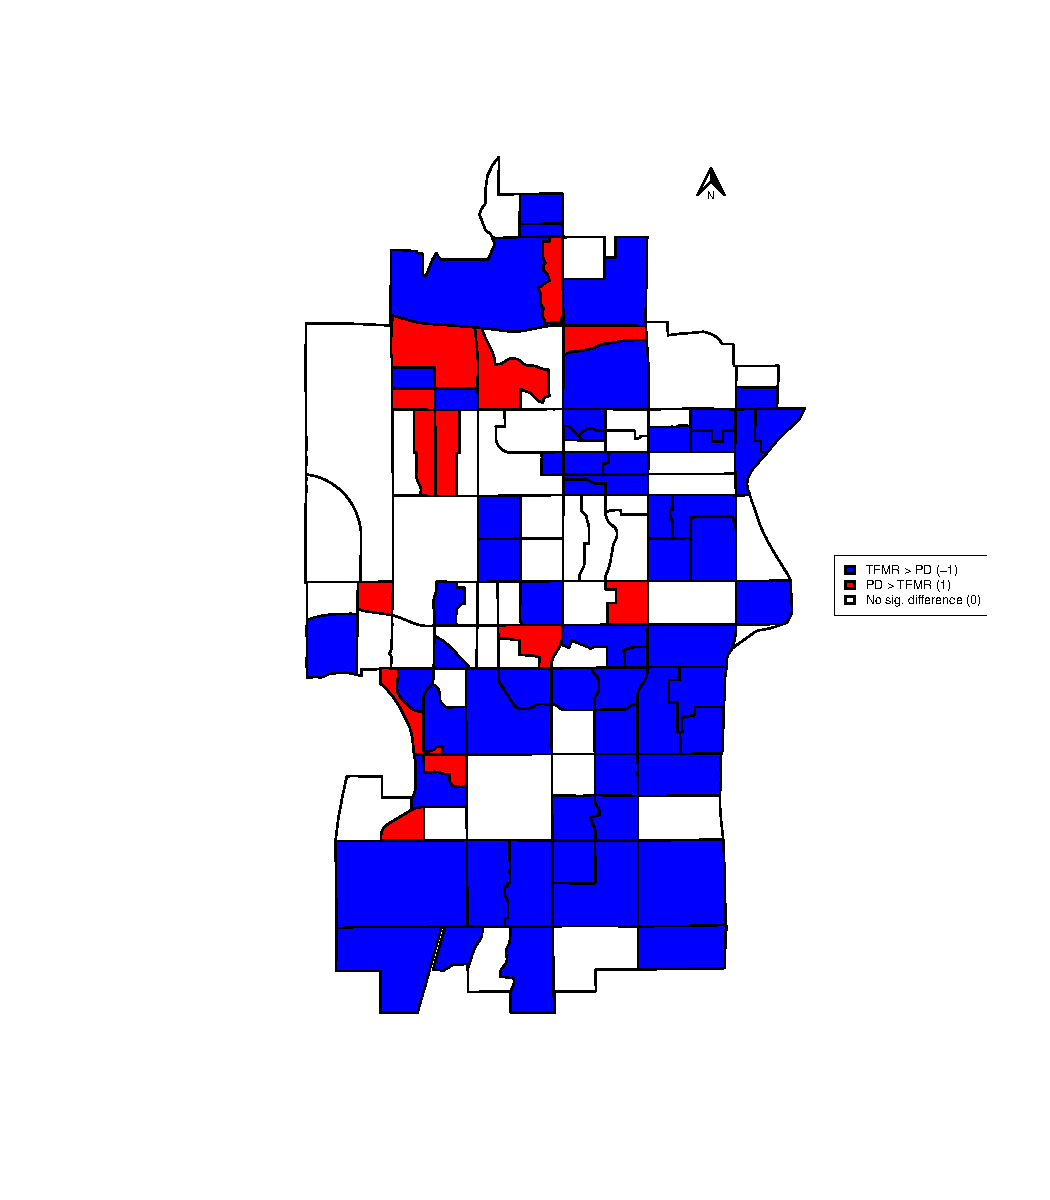
\includegraphics{figures/sppt-naloxone.pdf}
\end{figure}

\newpage

\begin{table}[htbp]\centering
\def\sym#1{\ifmmode^{#1}\else\(^{#1}\)\fi}
\caption{Mixed-effects Logistic Regression Models Predicting PD and TFMR first to Administer Naloxone}
\begin{adjustbox}{max width=\linewidth}\begin{tabular}{l*{2}{c}}
\toprule
                &\multicolumn{1}{c}{PD naloxone first}&\multicolumn{1}{c}{TFMR naloxone first}\\
\midrule
\emph{Independent variable}&                 &                 \\
Violent crime rate (per 1000)&0.997\sym{**} (0.001)        &1.001\sym{*} (0.001)        \\
\vspace{.05em} \\
Initial dispatch complaint (ref = Overdose/poisioning)&                 &                 \\
Health/medical related&0.684\sym{*} (0.104)        &1.326\sym{*} (0.182)        \\
Accidental injury&0.477 (0.502)        &0.770 (0.318)        \\
Public safety related&0.273 (0.282)        &0.519 (0.322)        \\
Mental health related&0.391\sym{**} (0.096)        &1.998\sym{**} (0.365)        \\
Other           &0.649\sym{**} (0.108)        &2.948\sym{**} (0.473)        \\
\vspace{.05em} \\
Female          &0.774 (0.127)        &1.126 (0.123)        \\
\vspace{.05em} \\
\emph{Block group predictors}&                 &                 \\
Violent crime spatial lag&1.008 (0.006)        &0.997 (0.004)        \\
Drug offense rate (per 1000)&1.007\sym{**} (0.002)        &0.994\sym{**} (0.002)        \\
Drug offense spatial lag&0.995 (0.007)        &1.005 (0.006)        \\
Opioid OD rate logged&0.937 (0.096)        &1.029 (0.087)        \\
Opioid OD spatial lag&0.996 (0.007)        &0.999 (0.006)        \\
\% Unemployed   &0.993 (0.012)        &0.999 (0.005)        \\
\% Residential land&1.001 (0.003)        &1.003 (0.002)        \\
\% Owner occupied units&0.978\sym{*} (0.009)        &0.995 (0.006)        \\
\% White        &1.012 (0.008)        &0.997 (0.005)        \\
\% Black        &1.025\sym{**} (0.007)        &0.987 (0.007)        \\
\% Hispanic     &1.007 (0.008)        &0.996 (0.006)        \\
Constant        &0.098\sym{**} (0.074)        &0.683 (0.355)        \\
\midrule
Random intercept&1.000\sym{**} (0.000)        &1.000 (0.000)        \\
\midrule
Observations    &     1,994        &     1,994        \\
Block groups    &  115        &  115        \\
AIC             & 1645.796        & 2464.457        \\
BIC             & 1830.527        & 2649.188        \\
\bottomrule
\multicolumn{3}{p{16cm}}{\footnotesize Exponentiated coefficients displayed. Clustered standard errors in parentheses. Month and year fixed effects included but not shown. Mean VIF value = 2.46, single highest VIF value = 7.49.}\\
\multicolumn{3}{l}{\footnotesize \sym{*} \(p<0.05\), \sym{**} \(p<0.01\), \sym{**} \(p<0.001\)}\\
\end{tabular} \end{adjustbox}
\end{table}


\newpage

\begin{figure}
    \caption{Coefficient Plot Predicting First to Administer Naloxone}
    \centering
    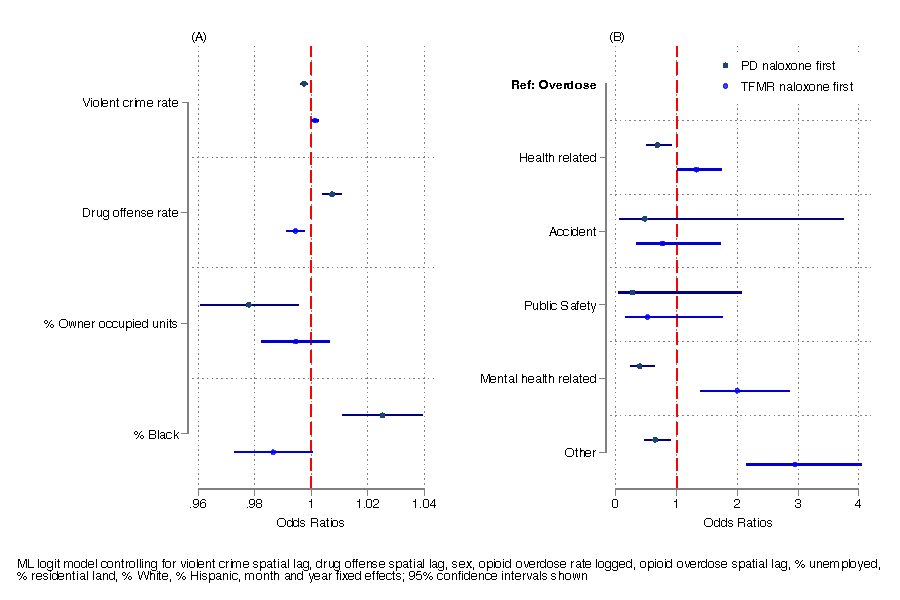
\includegraphics{figures/me-logit-coef-comb.pdf}
\end{figure}

\newpage 

\begin{table}[htbp]\centering
\def\sym#1{\ifmmode^{#1}\else\(^{#1}\)\fi}
\caption{Mixed-effects Logistic Regression Models Predicting PD and TFMR First to Administer Naloxone: PD and TFMR only}
\begin{adjustbox}{max width=\linewidth}\begin{tabular}{l*{2}{D{.}{.}{-1}}}
\toprule
                &\multicolumn{2}{c}{Police naloxone admin}\\\cmidrule(lr){2-3}
                &\multicolumn{1}{c}{(1)}        &\multicolumn{1}{c}{(2)}        \\
\midrule
\emph{Independent variable}&                 &                 \\
Violent crime rate (per 1000)&                 &0.995\sym{**} (0.001)        \\
\vspace{.05em} \\
Initial dispatch complaint (ref = Overdose/poisioning)&                 &                 \\
Health/medical related&                 &0.659\sym{*} (0.135)        \\
Accidental injury&                 &0.932 (1.005)        \\
Public safety related&                 &0.280 (0.193)        \\
Mental health related&                 &0.243\sym{**} (0.069)        \\
Other           &                 &0.347\sym{**} (0.072)        \\
\vspace{.05em} \\
Female          &                 &0.779 (0.149)        \\
\vspace{.05em} \\
Age range (ref = Aged 20 - 29)&                 &                 \\
Younger than 20 &                 &0.786 (0.279)        \\
Aged 30 - 39    &                 &0.881 (0.200)        \\
Aged 40 - 59    &                 &0.454\sym{**} (0.100)        \\
Aged 60 - 99    &                 &0.272\sym{**} (0.116)        \\
\vspace{.05em} \\
\emph{Block group predictors}&                 &                 \\
Violent crime spatial lag&                 &1.011 (0.007)        \\
Drug offense rate (per 1000)&                 &1.013\sym{**} (0.002)        \\
Drug offense spatial lag&                 &0.985\sym{*} (0.008)        \\
Opioid OD rate logged&                 &0.994 (0.149)        \\
Opioid OD spatial lag&                 &1.000 (0.001)        \\
Disadvantage&                 &1.079 (0.104)        \\
\% Residential land&                 &0.995 (0.003)        \\
\% Owner occupied units&                 &0.978 (0.013)        \\
\% White        &                 &1.024\sym{*} (0.011)        \\
\% Black        &                 &1.036\sym{**} (0.012)        \\
\% Hispanic     &                 &1.013 (0.010)        \\
Constant        &0.409\sym{**} (0.036)        &0.234 (0.263)        \\
\midrule
Random intercept&1.073 (0.067)        &1.000 (0.000)        \\
\midrule
Observations    &      955        &      891        \\
Block groups    &  112            &  106        \\
AIC             & 1170.921        & 1060.195        \\
BIC             & 1180.644        & 1381.282        \\
\bottomrule
\multicolumn{3}{p{20cm}}{\footnotesize Exponentiated coefficients; Clustered standard errors in parentheses; Day of month, month, and year fixed effects included but not shown; Mean VIF value = 2.30, single highest VIF value = 9.95. Reference group is now TFMR administering first -- Not all other observations.}\\
\multicolumn{3}{l}{\footnotesize \sym{*} \(p<0.05\), \sym{**} \(p<0.01\), \sym{**} \(p<0.001\)}\\
\end{tabular} \end{adjustbox}
\end{table}


\newpage
\begin{figure}
    \caption{Coefficient Plot Predicting First to Administer Naloxone: PD and TFMR only}
    \centering
    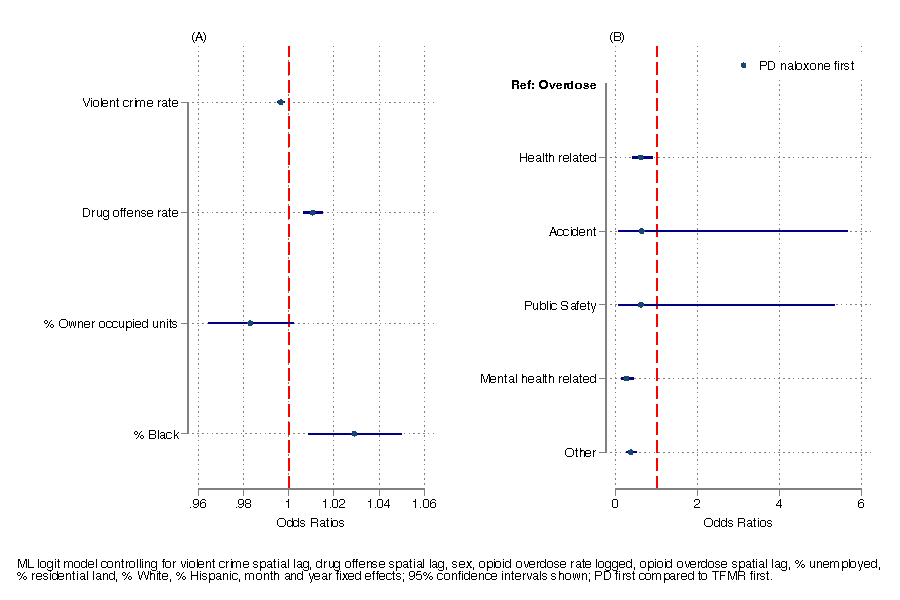
\includegraphics{figures/me-logit-coef-comb-sens.pdf}
\end{figure}
